
%Consider for instance the following scenario. An organization wants to provide the services' based application "To Publish Music" that monitors the music a person is listening during some periods of time and sends the song title  to this person's Twitter and Facebook accounts. Thus, this social network user will have her status synchronized in  Twitter and Facebook (i.e., either the same title is published in both accounts or it is not updated) with the title of the music she is listening in Spotify.
%For developing this services' based application it is necessary to compose the following services  calling  their  exported methods:
%\begin{itemize}
%\item The music service   Spotify exports a method for obtaining information  %about the music a given user is listening:
%%\begin{itemize} \item {\sf\small get-Last-Song ( userid ): String} ; %%\end{itemize}
%\item Facebook and Twitter services export a method for  updating the status of a given user:
%\begin{itemize} 
%%\item{\sf\small get-Status ( usedid ): String ; 
%\item {\sf\small update-Status ( userid, new-status ): String}; 
%\end{itemize}
%\end{itemize}
%
%Figure \ref{fig:E3valuemodel} shows the E3 value model \cite{e3value} of
%the scenario. The E3 value model is a business model that represents a business case graphically as a set of value exchanges ($\nabla$$\triangle$) and value activities (rounded boxes) performed by business actors (squared boxes) and allows us to understand the environment in which the services' composition will be placed. 
%The model in Figure \ref{fig:E3valuemodel} shows Spotify and a private application (which is also a service) that directly interact with users for providing free services for listening and publishing information about music being listened by users. The private application interacts with Spotify for obtaining free information about the flow of music being listened by a user in return of a fee (i.e., premium subscription). Finally, the private application interacts with Facebook and Twitter for updating the user's status and thereby they share non material benefits (i.e., the fact that users subscribe to their networks and are active on them thanks to the private application).

%Figure \ref{fig:E3valuemodel} shows the BPMN model  \footnote{Details on BPMN (Business Process Management Notation) can be found in http://www.bpmn.org/} of the scenario. 
%The "To Publish Music" scenario 
%%(showed by doted line) 
%starts by contacting the music service Spotify for retrieving the user's  musical status (activity {\sf Get Song}). 
%Twitter and Facebook services are then contacted in parallel for updating the user's status with the corresponding song title (activities {\sf Update Twitter} and {\sf Update Facebook}).
%\begin{figure}
%\centering
%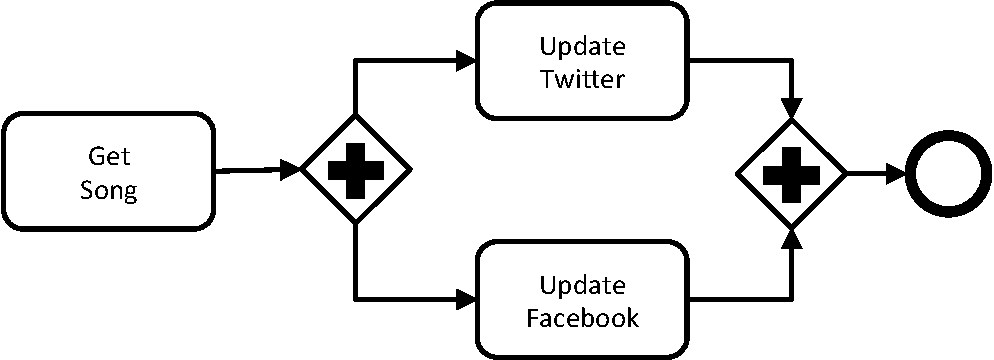
\includegraphics[width=0.55\textwidth]{figs/SC}
%\caption{BPMN model of the "To Publish Music" scenario}
%\label{fig:E3valuemodel}
%\end{figure}

In order to introduce the context of our work consider the Tracking crime application where civil population and by police share information about criminality in given zones of an imaginary city. 
Users signal crimes using twitter and police officers notify crimes  they have to deal with. 
Some of this information, if it is not confidential, can be shared to the community of users using this application. 
Users can track crimes in given zones and see information located in a map according to their privileges.  
For example civilians can ask Locate the crimes done the last month 100 km from my current position that happened between 8:00 and 14:00.
While police officers can ask Locate the regions in my sector where murders happened in the last month
This information can come from the police database and from twitter posts. 
The zones of the city are thereby according to their degree of criminality.

 In order to provide these functions the application benefits from existing services that provide information,  storage and data visualization functions. Thus, the application is a service based application that implements a business process.
 The business process is specified in terms of ordered tasks and define the application logic of a Service oriented Application. Tasks can be performed by a person or an entity. In our context, tasks are implemented by Services. 
Service is an application implemented by a provider that exports an API through a network (e.g., Internet)
API is defined using an interface definition language (IDL, e.g., WSDL for Web services).
 In our example the business procces can start with one of two tasks: Notify a crime, or track a crime. A notified crime can be then stored in a database. Tracked crimes are visualized in a map and then the used can ask for detailed information. They are implemented by four services: twitter and an adhoc police service for notifying crimes, Amazon as persistence service and google maps for visualizing and locating crimes in a map. 
Note that a task can be implemented by a service composition. This is the case of the task Notify crime in our example that enables to notify crimes through twitter or through the police notification service. 
 

Business processes have also associated rules and constraints that define their non functional requirements.  
NFR represents the “semantics” and the conditions in which the tasks must be done. 
In our example we have some constraints. 
\begin{itemize}
\item Twtter requires to be accessed through an authentication protocol, and the police crime notification service has a control  access protocol and allows only 3 tries to access it. 
\item Only users with enough privileges can store crimes’ notifications. 
\item Users can only track crimes notified by providers t that hey have authorization to contact; For example civil population cannot track all the crimes notified by the police. 
\item If the google map is unavailable the results of a track request are delivered on text. 
\item If a user tracks crimes that are provided by a service for which she does not have authorization then show an empty map. 
\item Detailed information about a crime depends on the user privileges, on the police assignment regions. 
\item The tracking crime app keeps track of the accesses to detailed information about crimes. 
\end{itemize}

Through the example we underlined that every application implements functional aspects that describe its application logic. Recall that an application logic refers to routines that perform the activities to reach the application objective.
Also there are non functional properties derived from NFR. They refer to strategies to be considered for the application execution like: security, isolation, adaptability, atomicity, and more.
These non functional properties must be ensured at execution time, and they are not completely defined within the application logic.

The challenge is to define them and to associate them with the application logic considering that different to existing solutions that suppose that it is possible to access the execution stat of all the components  of an application and that the application has complete control on them, in the case for service oriented applications  the components are autonomous services
API does not necessarily export information about methods dependency (e.g., in the REST protocol);
they do not share their state (stateless).






Given a set of services with their exported methods known in advance or provided by a  service directory, building services' based applications can be  a simple task that implies expressing an application logic as a services' composition. The challenge being  ensuring the compliance between the specification and the resulting application. Software engineering methods (e.g., \cite{1,2,decastro1,PapazoglouH06}) today can help to ensure this compliance, particularly when information systems include several sometimes complex business processes calling Web services or legacy applications exported as services. 

%..--..--..--..--..--..--..--..--..--..--..--..--..--..--..--..--..--..--..--..--..--..--..--..--..--..--..--..--..--..--..--..--..--..--..--..--..--..--
\subsection{Modeling a services' based application}
%..--..--..--..--..--..--..--..--..--..--..--..--..--..--..--..--..--..--..--..--..--..--..--..--..--..--..--..--..--..--..--..--..--..--..--..--..--..--
 Figure \ref{fig:sodm} shows  SOD-M that defines a service oriented approach   providing  a set of guidelines to build services' based information systems (SIS) \cite{decastro1,decastro2}.  Therefore, SOD-M proposes to use services as first-class objects for the whole process of the SIS  development and it  follows a Model Driven Architecture (MDA) \cite{miller}  approach. Extending from the highest level of abstraction of the MDA, SOD-M provides  a conceptual structure to: first, capture the system requirements and specification in high-level abstraction models (computation independent models, CIMÕs); next,  starting from such models build platform independent models (PIMÕs) specifying the system details; next transform such models into platform specific models (PSMÕs) that bundles the specification of the system with the details of the targeted platform; and finally, serialize such model into the working-code that implements the system. 
\begin{figure} [htpb]
\centering
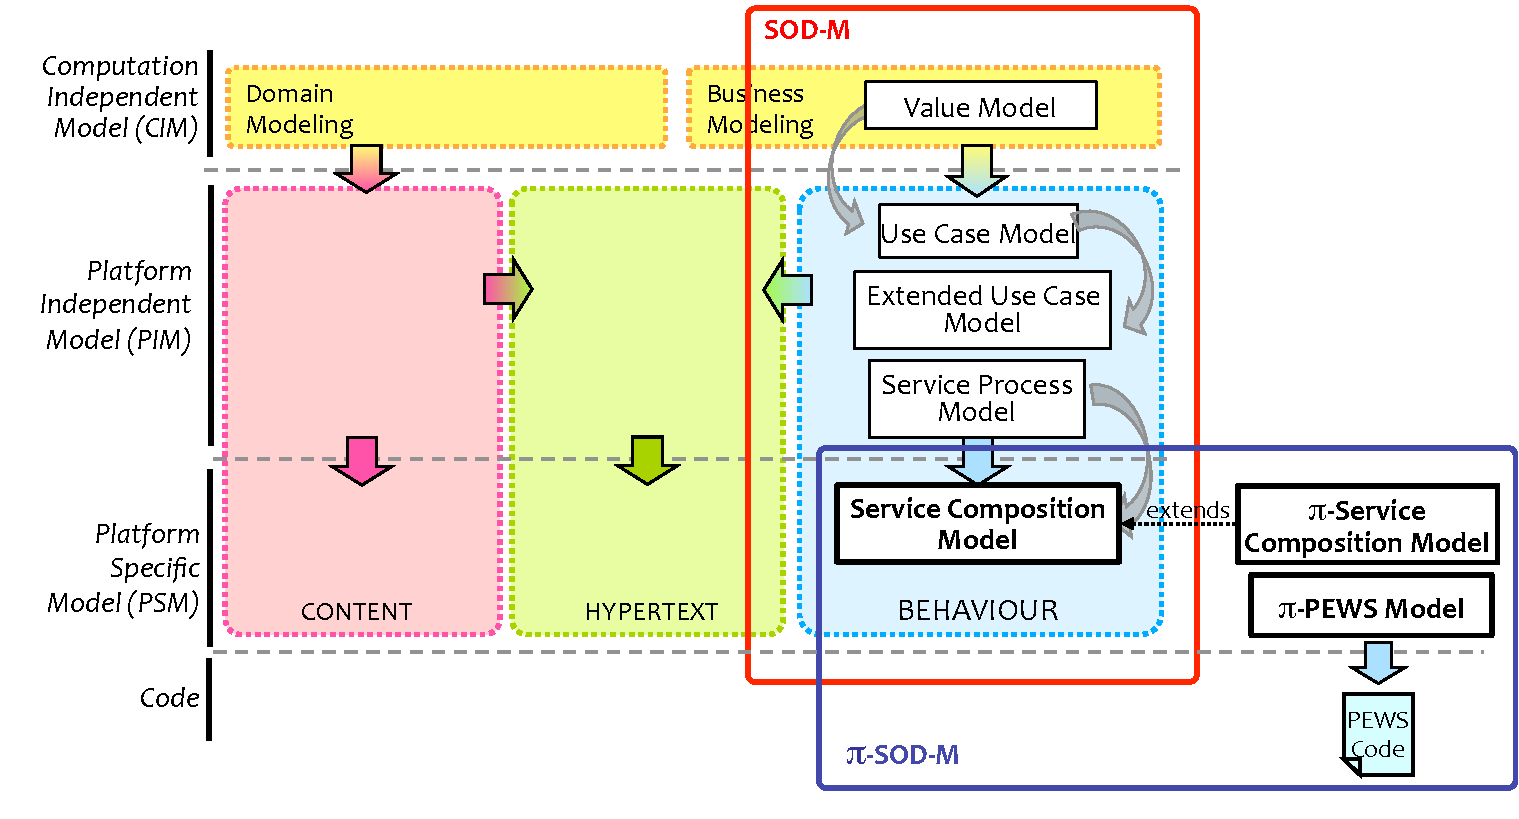
\includegraphics[width=0.65\textwidth]{figs/SODM}
\caption{SOD-M development process}
\label{fig:sodm}
\end{figure} 
As shown in Figure \ref{fig:sodm}, the SOD-M model-driven process begins by building the high-level computational independent models and enables specific models for a service platform to be obtained as a result  \cite{decastro1}. Referring to the "To Publish Music" application, using SOD-M the designer starts defining an E3value model \footnote{The E3 value model is a business model that represents a business case %graphically as a set of value exchanges ($\nabla$$\triangle$) and value activities (rounded boxes) performed by business actors (squared boxes) 
and allows  to understand the environment in which the services' composition will be placed \cite{e3value}.}  at the CIM level and then the corresponding models of the PIM are generated leading to a services' composition model (SCM).
%SOD-M proposes a set of models, :  i) the three different MDA abstraction levels: CIM, PIM and PSM; and ii) SOD-M views: business and information system views. 
%Model-Driven Engineering (MDE) \cite{schmidt} and particularly MDA \footnote{Model Driven Architecture (MDA)  is the particular model-driven proposal defined by the Object Management Group (OMG).} 
%provide
%is an evolving approach to software development that deals with the provision of 
%models, transformations between them and code generators to address software development. 
%One of the main advantages of model-driven approaches is the provision of 
%It also provides a conceptual structure where the models used by business managers and analysts can be traced towards more detailed models used by software developers.  

%Now, consider that besides the services' composition that represents the order in which the services are called for implementing the application "To Publish Music" it is necessary to model  other requirements that represent the (i) conditions imposed by services for being contacted, for example the fact the Facebook and Twitter require authentication protocol in order to call their methods for updating the wall; (ii) the conditions stemming from the business rules of the application logic, for example the fact that the walls in Facebook and Twitter must show the same song title and if this is not possible then none of them is updated. 

%..--..--..--..--..--..--..--..--..--..--..--..--..--..--..--..--..--..--..--..--..--..--..--..--..--..--..--..--..--..--..--..--..--..--..--..--..--..--
\subsection{Modeling non-functional constraints of services' based applications}
%..--..--..--..--..--..--..--..--..--..--..--..--..--..--..--..--..--..--..--..--..--..--..--..--..--..--..--..--..--..--..--..--..--..--..--..--..--..--
Adding non-functional requirements and services constraints in the services' composition is a complex task that implies programming  protocols for instance authentication protocols to call a service in our example, and atomicity (exception handling and recovery) for ensuring a true synchronization of the results produced by the service methods calls.
% song title disseminated in the walls of the user's Facebook and Twitter accounts. 

Service oriented computing promotes ease of information systems' construction thanks, for instance, to services' reuse. Yet, this is not applied to non-functional constraints as the ones described previously, because they do not follow in general the same service oriented principle and because they are often not fully considered in the specification process of existing services' oriented development methods. Rather, they   are either supposed to be ensured by the underlying execution platform, or they are programmed through ad-hoc protocols. Besides,  they are partially or rarely methodologically derived from the application specification, and they are added once the code has been implemented. In consequence, the resulting application does not fully preserve the compliance and reuse expectations provided by the service oriented computing methods.

%..--..--..--..--..--..--..--..--..--..--..--..--..--..--..--..--..--..--..--..--..--..--..--..--..--..--..--..--..--..--..--..--..--..--..--..--..--..--
%\subsection{$\pi$-SOD-M}
%..--..--..--..--..--..--..--..--..--..--..--..--..--..--..--..--..--..--..--..--..--..--..--..--..--..--..--..--..--..--..--..--..--..--..--..--..--..--

%
%Our proposal, called $\pi$-SOD-M, extends the services' composition model of the SOD-M method  with the notion of {\em A-Policy} \cite{Espinosa-Oviedo2011a} for representing services' composition constraints. 
%
Our work extends SOD-M for building applications by modeling the application logic and its associated non-functional constraints and thereby ensuring the generation of reliable services' composition. 
%This method is described in the following sections.
In order to do, our work organizes non-functional constraints into 
three layers representing: application modeling, services composition and services. The service composition layer serves as an integration layer between the services layer that exports methods and has associated constraints and characteristics; and the application layer that expresses requirements.
At the application layer NFP can refer to business rules and values. A value NFR expresses constraints about the way data and functions can be accessed and executed. For example accessing methods under security protocols.

Business NFP at the service layer concerns properties that are associated to services and defines how to call their exported operations (business properties). For example, response time, storage capacity (e.g., Dropbox service provides 5Giga free storage). Value constraints concern more on the conditions in which services can be used. For example, accessing to a function within an authentica-tion protocol.

Finally, at the service composition layer gives an abstract view of the kind of properties exported by services that can be combined for providing NFP for a composition. For example, confidentiality, authentication, privacy and access control can provide security at the service composition layer.

As a first step in our approach,  we started modeling non-functional constraints at the PSM level. Thus, in this paper we  propose the $\pi$-SCM, the services' composition meta-model extended with {\em A-policies} for modeling non-functional constraints (highlighted in Figure  \ref{fig:sodm} and described in Section \ref{sec:piscm}).  $\pi$-SOD-M defines the $\pi$-{\sc Pews}  meta-model providing guidelines for expressing the services' composition and the {\em A-policies} (see Section \ref{sec:pewsmetamodel}), and also defines model to model transformation rules for generating  $\pi$-{\sc Pews} models starting from $\pi$-SCM models that will support executable code generation (see Section \ref{sec:mmrules}). Finally, our work defines model to text transformation rules for generating the program that implements both the services' composition and the associated {\em A-policies} and that is executed by an adapted engine (see Section \ref{sec:implementation}).

